\chapter{Representing uncertainty} \label{ch:uncertainty}
This chapter will cover how we can represent uncertainty in vectors and Lie group elements in general using Gaussian \emph{probability distribution functions (PDFs)}.
We will also see how we can propagate uncertainty through functions of random variables.
This is a useful tool when we want to express uncertainty in different coordinate frames, or we want to propagate uncertainty through sensor models.
Most of this chapter is based on \cite{barfoot2017state, SolaARobotics, Mangelson2020CharacterizingAlgebra}.

\section{The multivariate normal distribution}
A \emph{multivariate normal} or \emph{Gaussian} PDF over the \emph{random variable} $\vecx \in \bbR^m$ can be expressed as
\begin{equation} \label{eq:multivarite-normal-pdf}
  p(\vecx; \bar{\vecx}, \matSigma) = \frac{1}{\sqrt{(2\pi)^m \det \matSigma}} \exp \left( -\frac{1}{2} (\vecx - \bar{\vecx})\trans \matSigma^{-1} (\vecx - \bar{\vecx}) \right),
\end{equation}
where the \emph{mean} $\bar{\vecx}$ is the expected value of $\vecx$,
\begin{equation} \label{eq:mean-def}
  \bar{\vecx} = \bbE[\vecx] \in \bbR^m,
\end{equation}
and the \emph{covariance matrix} $\matSigma$ is defined as the expected product of deviations
\begin{equation} \label{eq:cov-def}
  \matSigma = \bbE \left[(\vecx - \bar{\vecx}) (\vecx - \bar{\vecx})\trans \right] \in \bbR^{m \times m},
\end{equation}
where $\bbE[\cdot]$ is the \emph{expectation operator}.
We say that $\vecx$ is \emph{normally distributed} by using the notation
\begin{equation}
  \vecx \sim \cN(\bar{\vecx}, \matSigma),
\end{equation}
where $\cN(\bar{\vecx}, \matSigma)$ is shorthand for the PDF in \eqref{eq:multivarite-normal-pdf}.

The \emph{joint Gaussian distribution} over a pair of random variables, $(\vecx, \vecy)$, is given by
\begin{equation}
  p(\vecx, \vecy) = \cN \left(
  \begin{bmatrix}
    \bar{\vecx}\\
    \bar{\vecy}
  \end{bmatrix},
   \begin{bmatrix}
    \matSigma_{\vecx\vecx} & \matSigma_{\vecx\vecy}\\
    \matSigma_{\vecy\vecx} & \matSigma_{\vecy\vecy}
  \end{bmatrix} 
  \right),
\end{equation}
where $\matSigma_{\vecx\vecy} = \bbE [(\vecx - \bar{\vecx}) (\vecy - \bar{\vecy})\trans]$ and $\matSigma_{\vecy\vecx} = \matSigma_{\vecx\vecy}\trans$.
The convenient block structure of the joint covariance matrix lets us easily \emph{marginalise} the joint distribution to recover the two \emph{marginal Gaussian distributions}
\begin{align}
  p(\vecx) &= \cN(\bar{\vecx}, \matSigma_{\vecx\vecx})\\
  p(\vecy) &= \cN(\bar{\vecy}, \matSigma_{\vecy\vecy}). \label{eq:marginal-py}
\end{align}
It is also possible to break the joint distribution into the product of the two factors
\begin{equation}
  p(\vecx, \vecy) = p(\vecx | \vecy) p(\vecy),
\end{equation}
where the \emph{conditional distribution} of $\vecx$ given $\vecy$ is
\begin{equation} \label{eq:gaussian-conditional}
  p(\vecx | \vecy) = \cN(\bar{\vecx} + \matSigma_{\vecx\vecy}\matSigma_{\vecy\vecy}^{-1}(\vecy - \bar{\vecy}),\; \matSigma_{\vecx\vecx} - \matSigma_{\vecx\vecy}\matSigma_{\vecy\vecy}^{-1}\matSigma_{\vecy\vecx}),
\end{equation}
and the marginal distribution $p(\vecy)$ is given in \eqref{eq:marginal-py}.
The expression for the covariance of the conditional distribution, $\matSigma_{\vecx\vecx} - \matSigma_{\vecx\vecy}\matSigma_{\vecy\vecy}^{-1}\matSigma_{\vecy\vecx}$, is called the \emph{Schur complement} of $\matSigma_{\vecy\vecy}$.

Given a measurement $\vecy$, we can use \eqref{eq:gaussian-conditional} to update the distribution of $\vecx$ given the measurement by adjusting $\bar{\vecx}$ and reducing the uncertainty in $\matSigma_{\vecx\vecx}$. 
Or, equivalently, we can use the known joint distribution over state variables to represent all uncertainties relative to a given state.

\section{Uncertainty for Lie groups}
\begin{figure}[htb]
    \centering
    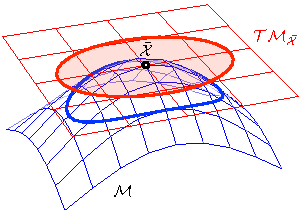
\includegraphics[width=0.6\columnwidth]{figures/covariance.pdf}
    \caption{Uncertainty around an element $\bar{\cX}$ on the manifold $\cM$ can be expressed as a covariance on the tangent vector space at the element (red).
    This lets us define a random variable on the tangent space that through perturbation with $\bar{\cX}$ induces the corresponding probability distribution on the manifold (blue).\\
    (Image source: \cite{SolaARobotics}; licensed under \href{https://creativecommons.org/licenses/by-nc-sa/4.0/}{CC BY-NC-SA 4.0})}
    \label{fig:uncertainty-on-manifold}
\end{figure}

We can represent a random variable on the manifold as a perturbation
\begin{equation}
  \cX = \bar{\cX} \oplus \vectau, \quad \vectau = \cX \ominus \bar{\cX},
\end{equation}
where $\bar{\cX} \in \cM$ is a nominal (noise-free) element, and $\vectau \in \bbR^m$ is a random variable in the tangent space $\cT\cM_{\bar{\cX}}$.
We can in this way define a PDF over $\vectau$ to induce a PDF on $\cX$.

Covariance matrices can be properly defined on $\cT\cM_{\bar{\cX}}$ with the expectation operator $\bbE[\cdot]$ as
\begin{equation}
  \matSigma_\cX = \bbE[\vectau \vectau\trans] = \bbE[(\cX \ominus \bar{\cX}) (\cX \ominus \bar{\cX})\trans] \in \bbR^{m \times m}.
\end{equation}
This lets us define the Gaussian PDF for the tangent space vector
\begin{equation}
  \vectau \sim \cN(\matr{0}, \matSigma_\cX),
\end{equation}
and the induced Gaussian PDF on the manifold (Figure~\ref{fig:uncertainty-on-manifold})
\begin{equation}
  \cX \sim \cN(\bar{\cX}, \matSigma_\cX).
\end{equation}

\begin{example}[frametitle=Drawing random poses from a Gaussian distribution]
Using the framework presented above, we can draw random poses from a distribution $\matT \sim \cN(\bar{\matT}, \matSigma_\matT)$ by perturbing the mean pose $\bar{\matT}$ with tangent vectors drawn from the distribution $\vecxi \sim \cN(\matr{0}, \matSigma_\matT)$, so that $\matT = \bar{\matT} \oplus \vecxi$.

{
  \centering
  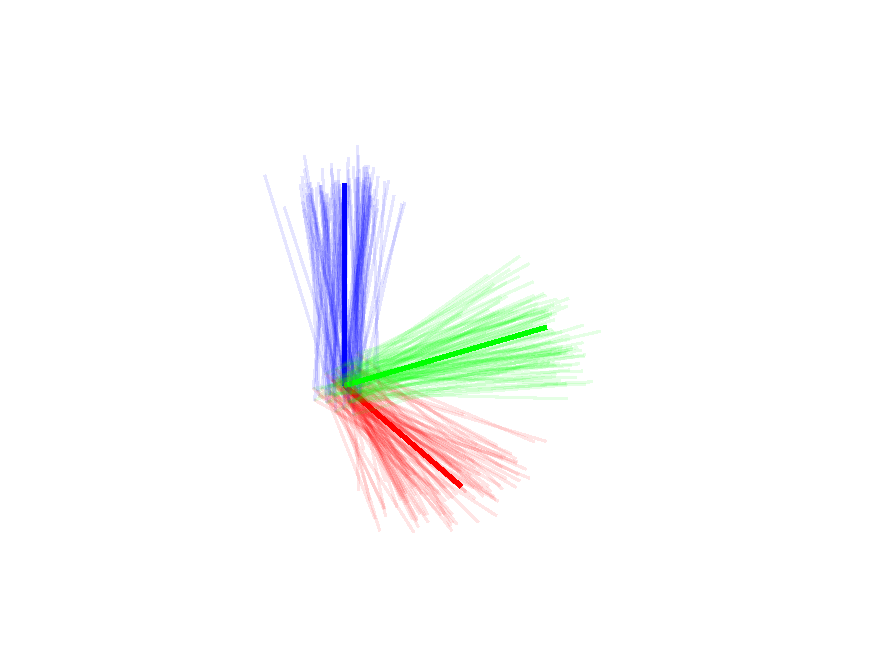
\includegraphics[width=0.75\columnwidth]{figures/draw-random-pose.pdf}
  \captionsetup{type=figure}
  \captionof{figure}{The mean pose $\bar{\matT}$ is shown in thick axes, while 50 poses drawn randomly from $\cN(\bar{\matT}, \matSigma_\matT)$ are shown in thin transparent axes.}
  \label{fig:draw-random-pose-example}
  \par
}

Figure~\ref{fig:draw-random-pose-example} shows the result of drawing 50 poses with $\bar{\matT} = \matI$ and

\begin{equation*}
  \matSigma_\matT =
  \begin{bmatrix}
    0.05 & & & & & \\
    & 0.05& & & & \\
    & & 0.05 & & & \\
    & & & 0.1 & & \\
    & & & & 0.1 & \\
    & & & & & 0.2 \\
  \end{bmatrix}.
\end{equation*}
\end{example}

It has been demonstrated that representing uncertainties on the manifold in this way captures the underlying distribution in stochastic kinematic models more accurately and more precisely, compared to representing uncertainties over position and orientation angles directly \cite{Long2012TheCoordinates}.

\begin{example}[frametitle=The banana distribution is Gaussian]
We will now demonstrate how a Gaussian PDF on the manifold lets us represent correlations between translation and orientation in a natural way with an experiment inspired from \cite{Long2012TheCoordinates}.

Consider an uncertain movement in the plane from the starting pose shown in black in Figure~\ref{fig:banana-distribution-example}.
Let the uncertain movement of 4 unit steps along the $x$-axis be represented by the stochastic 2D pose $\matT \in \SE(2)$, where $\matT \sim \cN(\bar{\matT}, \matSigma_\matT)$, and the uncertainty in translation along the $y$-axis and orientation are correlated:
\begin{equation*}
  \matSigma_\matT =
  \begin{bmatrix}
    0.1 & 0.0 & 0.0 \\
    0.0 & 2.0 & 0.4 \\
    0.0 & 0.4 & 0.1
  \end{bmatrix}.
\end{equation*}
We can visualise this distribution by transforming ellipsoids corresponding to constant probabilities to the plane by using the exponential map.
Figure~\ref{fig:banana-distribution-example} shows the probability contours corresponding to $75\%$ and $99\%$ in green, together with 100 randomly drawn poses from the same distribution.
Notice the distinct banana shape of the distribution in the plane, and how it fits with the clear correlation between position and orientation in the random pose samples.

{
  \centering
  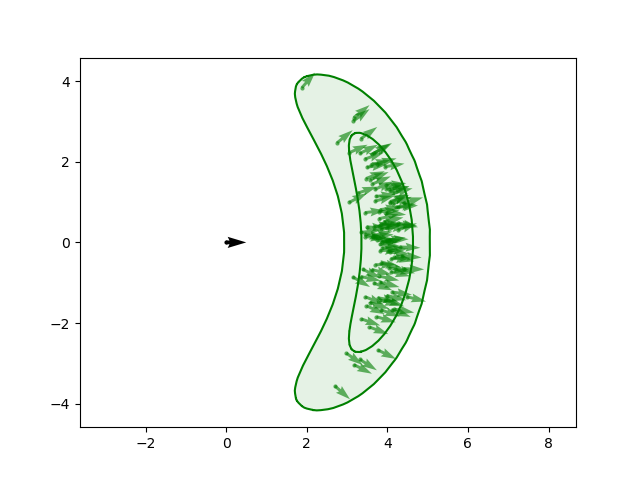
\includegraphics[width=0.75\columnwidth]{figures/banana-distribution.png}
  \captionsetup{type=figure}
  \captionof{figure}{The starting pose is shown as a black arrow, and the distribution representing the uncertain movement is visualised as filled green contours corresponding to $75\%$ and $99\%$ probabilities.
  100 pose samples drawn from the distribution are shown as green arrows.
  }
  \label{fig:banana-distribution-example}
  \par
}
\end{example}

\section{Propagation of uncertainty}
Let $f: \bbR^m \to \bbR^n$ be a function that takes the random variable $\vecx \in \bbR^m$ as input and produces the random variable $\vecy = f(\vecx) \in \bbR^n$ as output.
We will assume that $\vecx \sim \cN(\bar{\vecx}, \matSigma_\vecx)$.

Computing the uncertainty of the output $\vecy$ based on the effect of the uncertainties in the input $\vecx$ is sometimes called \emph{propagation of uncertainty}.
This is useful when we need to know the uncertainty in transformed variables, such as the uncertainty of poses in different coordinate frames, and the uncertainty in pixel position based on the uncertainty of a projected 3D point.

When $f(\vecx)$ is a linear function $\vecy = f(\vecx) = \matA\vecx + \vecb$, we can compute the probability distribution of $\vecy$ exactly.
Since the expectation operator is linear, we can compute the mean of $\vecy$ from the definition in \eqref{eq:mean-def} as
\begin{equation} \label{eq:linear-mean}
  \bar{\vecy} = \bbE[\vecy] = \bbE[\matA \vecx + \vecb] = \matA \bbE[\vecx] + \vecb = \matA \bar{\vecx} + \vecb = f(\bar{\vecx}).
\end{equation}
The covariance matrix of $\vecy$ is developed similarly from the definition in \eqref{eq:cov-def} by
\begin{subequations}\label{eq:linear-cov}
\begin{align}
  \matSigma_\vecy &= \bbE[(\vecy - \bar{\vecy}) (\vecy - \bar{\vecy})\trans]\\
  &= \bbE \left[  \left( (\matA \vecx + \vecb) - (\matA \bar{\vecx} + \vecb) \right) \left( (\matA \vecx + \vecb) - (\matA \bar{\vecx} + \vecb) \right)\trans \right]\\
  &= \bbE \left[ (\matA(\vecx - \bar{\vecx})) (\matA(\vecx - \bar{\vecx}))\trans \right]\\
  &= \bbE \left[ \matA(\vecx - \bar{\vecx}) (\vecx - \bar{\vecx})\trans \matA\trans \right]\\
  &= \matA \bbE\left[ (\vecx - \bar{\vecx}) (\vecx - \bar{\vecx})\trans \right] \matA\trans\\
  &= \matA \matSigma_\vecx \matA\trans.
\end{align}
\end{subequations}
The resulting probability distribution for $\vecy$ when $\vecy = f(\vecx)$ is linear is therefore given by
\begin{equation} \label{eq:linear-uncertainty-propagation}
  \vecy \sim \cN(f(\bar{\vecx}), \matA \matSigma_\vecx \matA\trans).
\end{equation}

\begin{example}[frametitle=Transforming random points with deterministic poses]
We are given the random 3D point $\vecx^c \sim \cN(\bar{\vecx}^c, \matSigma_{\vecx^c})$ in the camera frame $\cF_c$, and the \emph{deterministic} pose $\matT_{wc}$ of the camera frame relative to the world frame $\cF_w$.

Since $\vecx^w = \matT_{wc} \cdot \vecx^c = \matR_{wc}\vecx^c + \vect^w_{wc}$ is a linear function in $\vecx^c$, we can apply \eqref{eq:linear-uncertainty-propagation} to compute the exact distribution of the point in the world frame as
\begin{equation}
  \vecx^w \sim \cN(\matR_{wc}\bar{\vecx}^c + \vect^w_{wc}, \; \matR_{wc} \matSigma_{\vecx^c} \matR_{wc}\trans).
\end{equation}
\end{example}

For a random Lie group variable, $\cX \sim \cN(\bar{\cX}, \matSigma_\cX)$, since global and local perturbations are related linearly by the adjoint matrix \eqref{eq:adjoint-matrix}, we can transform the covariance matrices exactly between frames according to
\begin{equation}
  \prescript{\cE}{}{\matSigma}_\cX = \mAd_\cX \prescript{\cX}{}{\matSigma}_\cX {\mAd_\cX}\trans.
\end{equation}
This allows us to express the local distribution of $\cX$ exactly in the global frame.

For a \emph{nonlinear} function $g: \bbR^m \to \bbR^n$, where the random variable $\vecy$ is now given by $\vecy = g(\vecx)$, we will in general not get an exact Gaussian distribution over $\vecy$ when propagating the uncertainty of $\vecx$.
We can instead assume that $g(\vecx)$ is approximately linear around the mean of $\vecx$, so that we can use the propagation procedure above with the linear approximation.

We can linearise $g(\vecx)$ with a first order Taylor expansion \eqref{eq:linear-approximation} at the mean $\bar{\vecx}$ to get the linear form
\begin{equation} \label{eq:g-linearised}
  g(\vecx) = g(\bar{\vecx}  + (\vecx - \bar{\vecx})) \approx g(\bar{\vecx}) +  \jac{\vecy}{\bar{\vecx}}(\vecx - \bar{\vecx}),
\end{equation}
where the Jacobian is defined as
\begin{equation} \label{eq:noise-linearisation}
  \jac{\vecy}{\bar{\vecx}} \triangleq \dpar{g(\vecx)}{\vecx} \Bigr|_{\vecx = \bar{\vecx}}.
\end{equation}
Since $\bbE[\vecx - \bar{\vecx}] = \matr{0}$, developing the mean of \eqref{eq:g-linearised} according to \eqref{eq:linear-mean} gives us
\begin{equation}
  \bar{\vecy} \approx g(\bar{\vecx}).
\end{equation}
Developing the covariance matrix of \eqref{eq:g-linearised} according to \eqref{eq:linear-cov} results in
\begin{equation}
  \matSigma_\vecy \approx \jac{\vecy}{\bar{\vecx}}  \matSigma_\vecx \jac{\vecy}{\bar{\vecx}}\trans.
\end{equation}

We can therefore propagate the uncertainty through the nonlinear function $g(\vecx)$ by approximating it locally as a linear function $g(\bar{\vecx}) +  \jac{\vecy}{\bar{\vecx}}(\vecx - \bar{\vecx})$ to get the approximate PDF for $\vecy = g(\vecx)$ as
\begin{equation}
  \vecy \sim \cN(g(\bar{\vecx}), \jac{\vecy}{\bar{\vecx}}  \matSigma_\vecx \jac{\vecy}{\bar{\vecx}}\trans).
\end{equation}

It is also possible to perform uncertainty propagation using higher order approximations \cite{barfoot2017state}.

\begin{example}[frametitle=Uncertainty in backprojection] \label{ex:uncertainty-backrpojection}
Given a calibrated camera with intrinsic matrix
\begin{equation}
  \matK =
    \begin{bmatrix}
    f_u & 0 & c_u\\
    0 & f_v & c_v\\
    0 & 0 & 1
  \end{bmatrix},
\end{equation}
we can use the inverse perspective camera model,
\begin{equation}
  \vecx^c = \pi^{-1}(\vecu, z) = z \matK^{-1}
  \breve{\vecu}
  = z
  \begin{bmatrix}
   \frac{u - c_u}{f_u}\\[1em]
   \frac{v - c_v}{f_v}\\[1em]
    1
  \end{bmatrix},
\end{equation}
to compute the 3D point $\vecx^c$ in the camera frame that corresponds to a pixel $\vecu$ with depth $z$.
Given the pose $\matT_{wc}$ of the camera relative to the world frame, we get the corresponding world point from $\vecx^w = \matT_{wc} \cdot \vecx^c$.
This gives us the model
\begin{equation}
  \vecx^w = f(\matT_{wc}, \vecu, z) = \matT_{wc} \cdot \pi^{-1}(\vecu, z).
\end{equation}

We are given the parameters for the model as random variables
\begin{align}
  \matT_{wc} &\sim \cN(\bar{\matT}_{wc}, \matSigma_{\matT_{wc}})\\
  \vecu &\sim \cN(\bar{\vecu}, \matSigma_{\vecu})\\
  z &\sim \cN(\bar{z}, \sigma^2_z).
\end{align}

We can approximate the distribution for the backprojected point as
\begin{align}
  \bar{\vecx}^w &= f(\bar{\matT}_{wc}, \bar{\vecu}, \bar{z}) \label{eq:est_x}\\
  \matSigma_{\vecx^w} &= \jac{f}{\bar{\matT}_{wc}} \matSigma_{\matT_{wc}} {\jac{f}{\bar{\matT}_{wc}}}\trans +
  \jac{f}{\bar{\vecu}} \matSigma_{\vecu} \jac{f}{\bar{\vecu}}\trans +
  \jac{f}{\bar{z}} \sigma^2_z {\jac{f}{\bar{z}}}\trans. \label{eq:est_S}
\end{align}
Using the Jacobian blocks from section \ref{sec:Jacobians-SE3}, we get the Jacobians
\begin{align}
  \jac{f}{\bar{\matT}_{wc}} &= \jac{\bar{\matT}_{wc} \cdot \pi^{-1}}{\bar{\matT}_{wc}} = \jac{\bar{\matT}_{wc} \cdot \vecx^c}{\bar{\matT}_{wc}} = 
  \begin{bmatrix}
    \bar{\matR}_{wc} & -\bar{\matR}_{wc} \; [\vecx^c]_\times
  \end{bmatrix}\\[1em]
  \jac{f}{\bar{\vecu}} &= \jac{\bar{\matT}_{wc} \cdot \pi^{-1}}{\pi^{-1}} \jac{\pi^{-1}}{\bar{\vecu}} = \bar{\matR}_{wc}
    \begin{bmatrix}
    \frac{\bar{z}}{f_u} & 0\\
    0 & \frac{\bar{z}}{f_v}\\
    0 & 0
  \end{bmatrix}\\[1em]
  \jac{f}{\bar{z}} &= \jac{\bar{\matT}_{wc} \cdot \pi^{-1}}{\pi^{-1}} \jac{\pi^{-1}}{\bar{z}} = \bar{\matR}_{wc} \; \matK^{-1} \breve{\bar{\vecu}},
\end{align}
which allows us to compute the approximation $\vecx^w \sim \cN(\bar{\vecx}^w, \matSigma_{\vecx^w})$.
\end{example}

\section{Propagating uncertainty with Lie operations}
We will here (temporarily very briefly) present the main results from \cite{Mangelson2020CharacterizingAlgebra}, which lets us propagate uncertainty through important operations on Lie elements by also taking correlations into account.
The original paper is based on left perturbations, so we will here present the corresponding results for right perturbations.
See Appendix~\ref{ch:app-prop-lie-operations} for details.

\subsection{The inverse operation}
Given the distribution $\cX_{ij} \sim \cN(\bar{\cX}_{ij}, \matSigma_{\cX_{ij}})$, the corresponding distribution of the inverse element $\cX_{ji} = \cX_{ij}^{-1}$ is given by $\cX_{ji} \sim \cN(\bar{\cX}_{ji}, \matSigma_{\cX_{ji}})$, where these are exactly given as
\begin{align}
    \bar{\cX}_{ji} & = \bar{\cX}_{ij}^{-1}\\
    \matSigma_{\cX_{ji}} &= \mAd_{\bar{\cX}_{ij}} \matSigma_{\cX_{ij}} \mAd_{\bar{\cX}_{ij}}\trans.
\end{align}

\subsection{The composition operation}
Given the joint distribution over $[\cX_{ij}, \cX_{jk}]$, the distribution over the composition $\cX_{ik} = \cX_{ij} \circ \cX_{jk}$ is given to first order by
\begin{align}
    \bar{\cX}_{ik} &= \bar{\cX}_{ij} \circ \bar{\cX}_{jk}\\
    \matSigma_{\cX_{ik}} &\approx 
    \mAd_{\bar{\cX}_{jk}^{-1}} \matSigma_{\cX_{ij}} \mAd_{\bar{\cX}_{jk}^{-1}}\trans \nonumber\\
    &+ \matSigma_{\cX_{jk}} \nonumber\\
    &+ \mAd_{\bar{\cX}_{jk}^{-1}} \matSigma_{\cX_{ij}, \cX_{jk}}\\
    &+ \matSigma_{\cX_{jk}, \cX_{ij}} \mAd_{\bar{\cX}_{jk}^{-1}}\trans \nonumber
\end{align}

\subsection{The relative composition}
Given the joint distribution over $[\cX_{ij}, \cX_{ik}]$, the distribution over the relative composition $\cX_{jk} = \cX_{ij}^{-1} \circ \cX_{ik}$ is given to first order by
\begin{align}
  \bar{\cX}_{jk} &= \bar{\cX}_{ij}^{-1} \circ \bar{\cX}_{ik}\\
  \matSigma_{\cX_{jk}} &\approx 
  \mAd_{\bar{\cX}_{jk}^{-1}} \matSigma_{\cX_{ij}} \mAd_{\bar{\cX}_{jk}^{-1}}\trans \nonumber\\
    &+ \matSigma_{\cX_{ik}} \nonumber\\
    &- \mAd_{\bar{\cX}_{jk}^{-1}} \matSigma_{\cX_{ij}, \cX_{ik}}\\
    &- \matSigma_{\cX_{ik}, \cX_{ij}} \mAd_{\bar{\cX}_{jk}^{-1}}\trans \nonumber
\end{align}
